\documentclass[12pt]{article}

\title{Side Project Summary 2017--2019}
\author{William John Holden}
\date{\today}

\usepackage{amsmath,amsthm}
\usepackage{mathtools}
\usepackage{parskip}
\usepackage{amssymb}
\usepackage[margin=1.0in]{geometry}
\usepackage{minted}
\usepackage[utf8x]{inputenc}
\usepackage[hyphens]{url}
\usepackage[hidelinks]{hyperref}
\usepackage{listings}
\lstset{basicstyle=\ttfamily,columns=flexible,frame=single,breaklines=true}
\usepackage{graphicx}

\begin{document}
\maketitle

\begin{abstract}
At 2017--2019 job I worked on several side projects.
I hope that these programs will be useful to others after I leave.
This document catalogs the purpose, capability, and usage of each program.
Only projects that were written directly in support of my job are listed here.
None of these programs require privileged access or installation, although host-based firewalls may interfere with network-aware programs.
\end{abstract}

\section{Connection Map}

\textbf{Location}: \url{https://github.com/wjholden/Connection-Map}

\textbf{Input}: Syslog messages on UDP port 514 from a Cisco ASA.

\textbf{Output}: World map with TCP/UDP connections plotted to their estimated geographical location (see figure \ref{fig:connection-map}).

\textbf{Language}: Java

\begin{figure}[h]
\centering
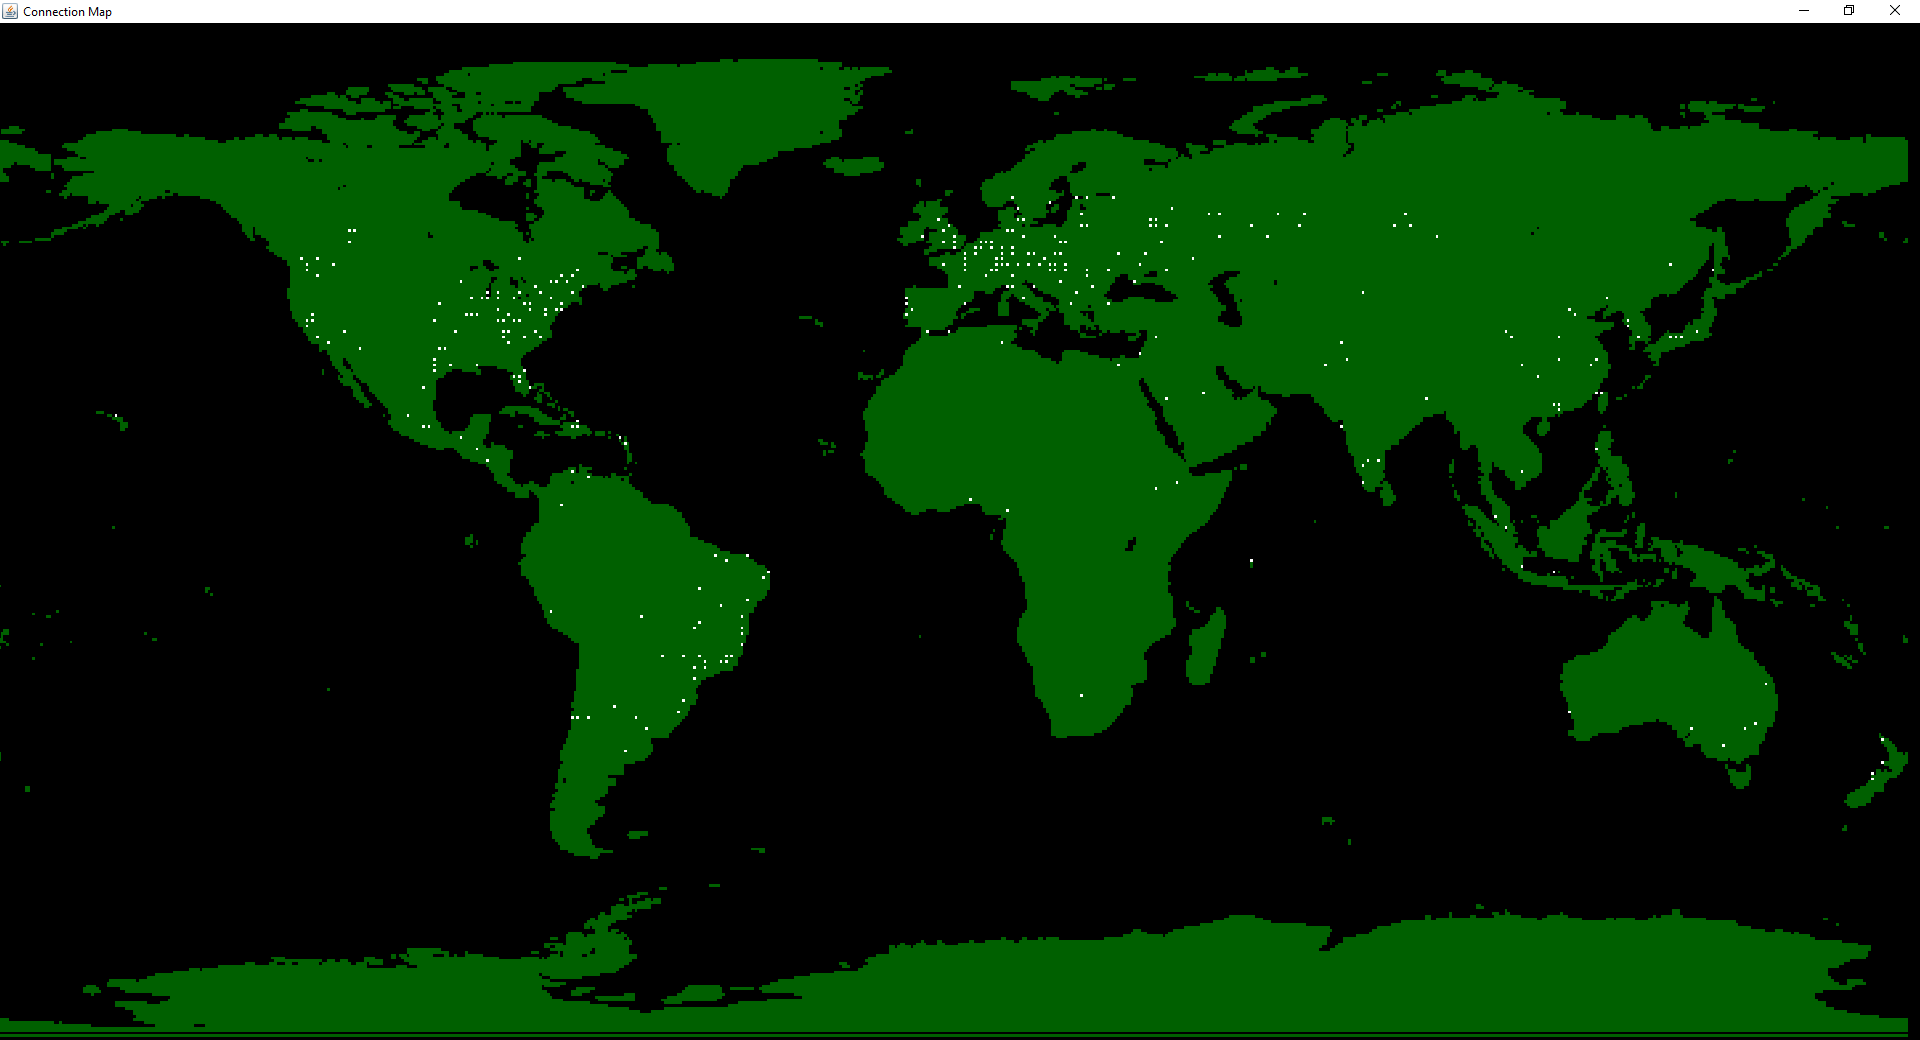
\includegraphics[width=\textwidth]{Connection-Map}
\caption{Connection Map}
\label{fig:connection-map}
\end{figure}

Connection Map is a Java 8 program to visualize network connections through a Cisco ASA firewall on a map. It uses the GeoLite2 ``GeoIP'' database available from \url{https://www.maxmind.com}.

Download the entire project from GitHub with the ``Clone or download'' button and select ``Download ZIP.'' Execute the runnable JAR \texttt{Connection-Map/Connection\_Map.jar}. The \texttt{Connection-Map/lib/} folder must be present and must contain all dependencies.

Press \texttt{h} for ``help'' inside the program.

Connection Map passively listens on UDP port 514 for Syslog messages. The program actually opens UDP port 514 as a multicast on the non-standard group \texttt{239.5.1.4}. Connection Map does not allow the operator to select which network interface it will bind to; binding decisions are left to the operating system. Microsoft Windows may bind the socket to an unexpected network interface. Use the command \texttt{netsh interface ipv4 show join} to observe which network interface the socket bound to. Npcap (included with Wireshark) may install a \texttt{Npcap Loopback Adapter} interface and VMware may install a \texttt{VMnet1} interface. These interfaces may have a faster ``speed'' and therefore lower route metric than the physical Ethernet and Wi-Fi interfaces (see \url{https://github.com/nmap/nmap/issues/1605}). If \texttt{netsh interface ipv4 show join} shows that \texttt{239.5.1.4} is joined on the incorrect interface, try disabling the other interface or change its metric (\texttt{Set-NetRoute}).

To configure a Cisco ASA to send Syslog messages to the Connection Map monitoring station, simply input the following commands in global configuration mode:

\begin{lstlisting}
logging enable
logging trap debugging
logging host inside x.x.x.x
\end{lstlisting}

\texttt{x.x.x.x} is either the unicast IP address of the monitoring station or \texttt{239.5.1.4}. The Connection Map program uses regular expressions to find Syslog messages 302013, 302014, 302015, and 302016 (see \url{https://www.cisco.com/c/en/us/td/docs/security/asa/syslog/b_syslog/syslogs3.html}). It assumes the external interface is named \texttt{outside} (case-sensitive). The name of the external interface is not configurable; if the name of the internal interface is not \texttt{outside} then the source code must be modified.

This program may be compatible with Cisco Firepower (see \url{https://www.cisco.com/c/en/us/td/docs/security/firepower/Syslogs/b_fptd_syslog_guide/syslogs3.html}).

\section{lsdb.js}

\textbf{Location}: \url{https://github.com/wjholden/lsdb.js}

\textbf{Input}: OSPF LSDB gathered by \texttt{snmpwalk}.

\textbf{Output}: OSPF LSDB in both DOT format and in graphical format (see figure \ref{fig:lsdb}).

\textbf{Language}: JavaScript

\begin{figure}[h]
\centering
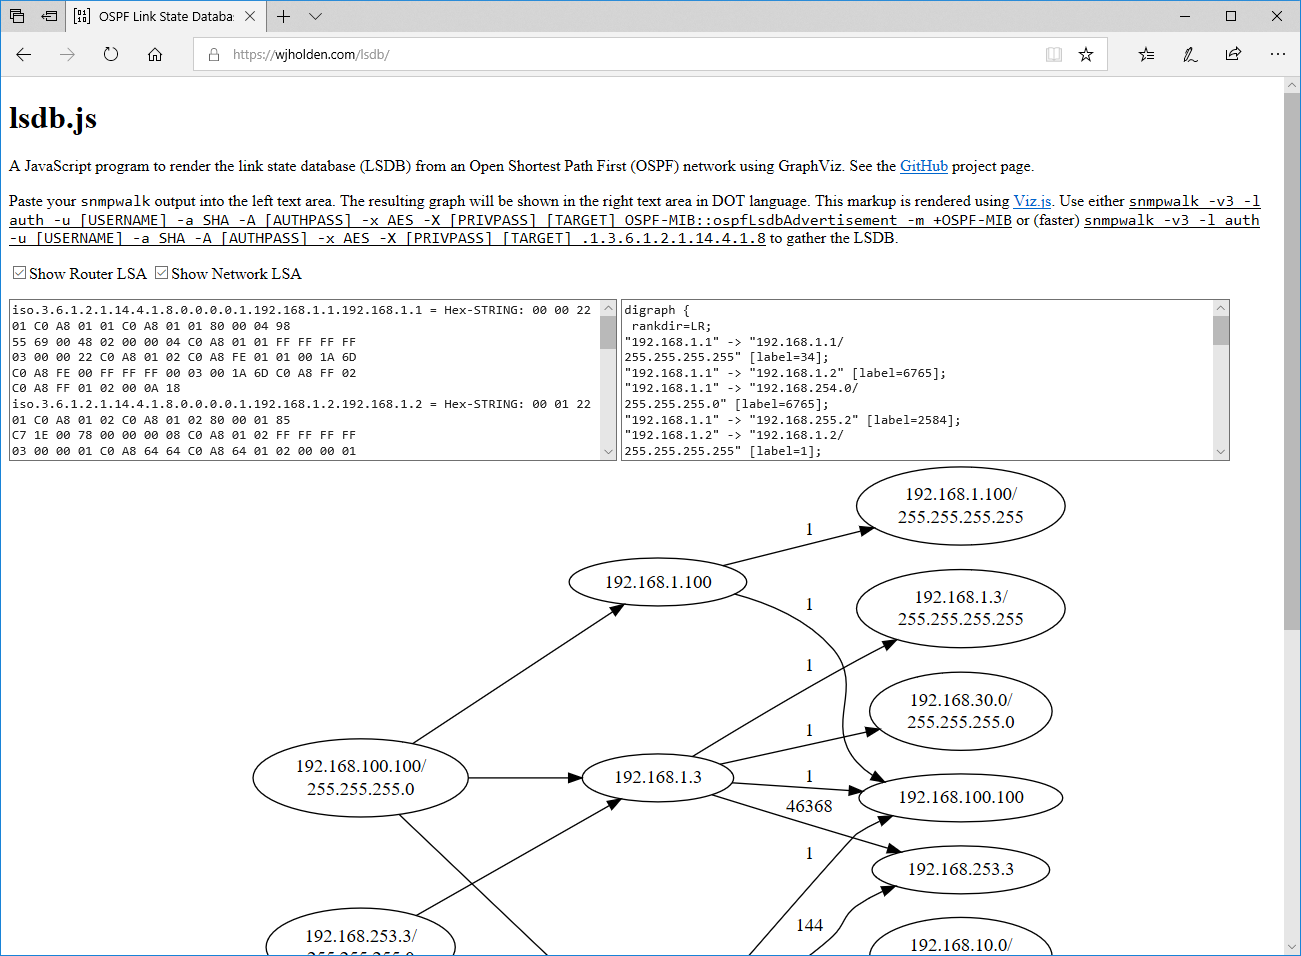
\includegraphics[width=\textwidth]{lsdb.PNG}
\caption{lsdb.js}
\label{fig:lsdb}
\end{figure}

lsdb.js is a derivative of an earlier Python program, Area Monitor (\url{https://github.com/wjholden/Area-Monitor}). Area Monitor began as an effort to peer with OSPF routers over IP protocol number 89. My first experiment with such low-level programming was in a C program (\url{https://github.com/wjholden/hello-ospf}). Low-level network programming is very difficult. After significant research and experimentation, I realized that you can get the LSDB in its entirety directly from a router using SNMP.

The \texttt{snmpwalk} command is an easy and useful method to gather the LSDB. Either of the following commands are sufficient to gather the LSDB over SNMPv3. Use the latter if the OSPF-MIB is not available to \texttt{snmpwalk}.

\begin{lstlisting}
snmpwalk -v3 -l auth -u [USERNAME] -a SHA -A [AUTHPASS] -x AES -X [PRIVPASS] [TARGET] OSPF-MIB::ospfLsdbAdvertisement -m +OSPF-MIB
snmpwalk -v3 -l auth -u [USERNAME] -a SHA -A [AUTHPASS] -x AES -X [PRIVPASS] [TARGET] .1.3.6.1.2.1.14.4.1.8
\end{lstlisting}

Paste the output from \texttt{snmpwalk} into the left text area. The lsdb.js program is hosted at \url{https://wjholden.com/lsdb/}, but the project can be copied anywhere (including local folders) and still work.

lsdb.js translates the link state database to the DOT format used by GraphViz. The program can interpret router and network link state advertisements (LSAs). These LSAs may be switched on or off by toggling the checkboxes shown in the web page. The DOT output is shown in the second text area.

Finally, lsdb.js calls Viz.js (\url{http://viz-js.com/}), an emscripten (\url{https://emscripten.org}) build of Graphviz (\url{https://www.graphviz.org}), to render the DOT output as an image. This image is shown in the web page.

Operators may edit the text in both text areas to customize their graphic.

The layout of network diagrams is generally less than beautiful. The network diagrams generated might be useful to:

\begin{itemize}
	\item Get started with a network diagram. Assign vertices to subgraphs and manually adjust their ordering of the vertices to find an appealing arrangement.
	\item Change detection. Run \texttt{snmpwalk} as a scheduled task on a regular basis. Store the output for later use in ``spot-the-differences'' troubleshooting.
	\item Discover mismatched interface costs. An interesting design feature (design flaw?) of OSPF is that interface costs may be mismatched. For example, routers R1, R2, and R3 may each be connected to the same broadcast network, but their the \texttt{ip ospf cost} configuration can be unequal. Unequal link costs may cause asymmetric routing. Link costs are shown as edge labels.	
\end{itemize}

\section{Node Monitor}

\textbf{Location}: \url{https://github.com/wjholden/Node-Monitor}

\textbf{Input}: 

\textbf{Output}: 

\textbf{Language}: Java


\section{Route Monitor}

\textbf{Location}: \url{https://github.com/wjholden/Route-Monitor}

\textbf{Input}: one or more network addresses, subnet masks, and network descriptions as command-line arguments

\textbf{Output}: 

\textbf{Language}: Java


\section{Key Chain Generator}

\textbf{Location}: \url{https://wjholden.com/keychain}

\textbf{Input}: None.

\textbf{Output}: 

\textbf{Language}: JavaScript



\section{CommSync II Output Interpreter}

\textbf{Location}: \url{https://wjholden.com/commsync}

\textbf{Input}: 

\textbf{Output}: 

\textbf{Language}: JavaScript




\end{document}